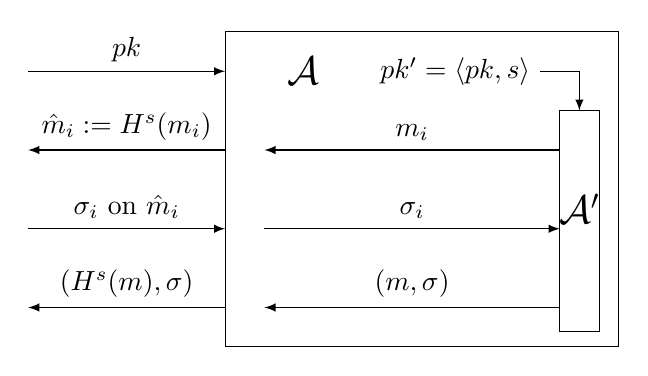
\begin{tikzpicture}
\draw (0,0) rectangle (5,4);
\draw (4.25,0.2) rectangle (4.75,3);
\draw[-latex] (-2.5,3.5) -- (0,3.5) node [midway, above] {$pk$};
\draw[-latex] (0,2.5) -- (-2.5,2.5) node [midway, above] {$\hat{m}_i := H^s(m_i)$};
\draw[-latex] (-2.5,1.5) -- (0,1.5) node [midway, above] {$\sigma_i$ on $\hat{m}_i$};
\draw[-latex] (0,0.5) -- (-2.5,0.5) node [midway, above] {$(H^s(m),\sigma)$};
\draw (1,3.5) node {{\Large $\mathcal{A}$}};
\draw[-latex] (4,3.5) node [left] {$pk' = \langle pk,s\rangle$} -| (4.5,3);
\draw (4.5,1.75) node {\Large $\mathcal{A}'$};
\draw[-latex] (4.25,2.5) -- (0.5,2.5) node [midway, above] {$m_i$};
\draw[-latex] (0.5,1.5) -- (4.25,1.5) node [midway, above] {$\sigma_i$};
\draw[-latex] (4.25,0.5) -- (0.5,0.5) node [midway, above] {$(m,\sigma)$};
%\draw[-latex] (4.5,3.5) node[above] {$pk$} -- (4.5,3);
\end{tikzpicture}